\documentclass[12pt]{article}
    \title{\textbf{Monitoraggio temperatura forno solare e controllo automatico orientamento specchi}}
    \author{Scar. Francesco}
    \date{}
    \addtolength{\topmargin}{-2cm}
    \addtolength{\textheight}{3cm}
    \renewcommand{\contentsname}{Contenuti}
    \renewcommand{\figurename}{Fig.}
    \newenvironment{changemargin}[2]{%
    \begin{list}{}{%
    \setlength{\topsep}{0pt}%
    \setlength{\leftmargin}{#1}%
    \setlength{\rightmargin}{#2}%
    \setlength{\listparindent}{\parindent}%
    \setlength{\itemindent}{\parindent}%
    \setlength{\parsep}{\parskip}%
    }%
    \item[]}{\end{list}}
    \long\def\/*#1*/{}          % Multiline comments https://tex.stackexchange.com/questions/87303/multi-line-block-comments-in-latex
    \usepackage{pdfpages}
    \usepackage{listings}
    \usepackage[utf8]{inputenc}
    \usepackage[T1]{fontenc}
    \usepackage{textcomp}
    \usepackage{gensymb}
    \usepackage{typearea}
    \usepackage[utf8]{inputenc}
    \usepackage[T1]{fontenc}
    \usepackage{color}
    \usepackage{mwe}
    \usepackage{listings}    
    \usepackage{etoolbox}
    \usepackage{amsmath}
    \usepackage{graphicx}
    \usepackage[hidelinks]{hyperref}
    
    \definecolor{mygreen}{rgb}{0,0.6,0}
    \definecolor{mygray}{rgb}{0.47,0.47,0.33}
    \definecolor{myorange}{rgb}{0.8,0.4,0}
    \definecolor{mywhite}{rgb}{0.98,0.98,0.98}
    \definecolor{myblue}{rgb}{0.01,0.61,0.98}
    

    \newcommand*{\FormatDigit}[1]{\ttfamily\textcolor{mygreen}{#1}}
    %% https://tex.stackexchange.com/questions/32174/listings-package-how-can-i-format-all-numbers
    \lstdefinestyle{FormattedNumber}{%
        literate=*{0}{{\FormatDigit{0}}}{1}%
                 {1}{{\FormatDigit{1}}}{1}%
                 {2}{{\FormatDigit{2}}}{1}%
                 {3}{{\FormatDigit{3}}}{1}%
                 {4}{{\FormatDigit{4}}}{1}%
                 {5}{{\FormatDigit{5}}}{1}%
                 {6}{{\FormatDigit{6}}}{1}%
                 {7}{{\FormatDigit{7}}}{1}%
                 {8}{{\FormatDigit{8}}}{1}%
                 {9}{{\FormatDigit{9}}}{1}%
                 {.0}{{\FormatDigit{.0}}}{2}% Following is to ensure that only periods
                 {.1}{{\FormatDigit{.1}}}{2}% followed by a digit are changed.
                 {.2}{{\FormatDigit{.2}}}{2}%
                 {.3}{{\FormatDigit{.3}}}{2}%
                 {.4}{{\FormatDigit{.4}}}{2}%
                 {.5}{{\FormatDigit{.5}}}{2}%
                 {.6}{{\FormatDigit{.6}}}{2}%
                 {.7}{{\FormatDigit{.7}}}{2}%
                 {.8}{{\FormatDigit{.8}}}{2}%
                 {.9}{{\FormatDigit{.9}}}{2}%
                 %{,}{{\FormatDigit{,}}{1}% depends if you want the "," in color
                 {\ }{{ }}{1}% handle the space
                 ,%
    }


    \lstset{%
      backgroundcolor=\color{mywhite},   
      basicstyle=\footnotesize,       
      breakatwhitespace=false,         
      breaklines=true,                 
      captionpos=b,                   
      commentstyle=\color{gray},    
      deletekeywords={...},           
      escapeinside={\%*}{*)},          
      extendedchars=true,              
      frame=single,                    
      keepspaces=true,                 
      keywordstyle=\color{myorange},       
      language=c++,                
      morekeywords={*,...},            
      numbers=left,                   
      numberstyle=\tiny\color{mygray}, 
      rulecolor=\color{black},         
      rulesepcolor=\color{myblue},
      showspaces=false,                
      showstringspaces=false,          
      showtabs=false
      stringstyle=\color{green},    
      tabsize=2,
      emphstyle=\bfseries\color{blue},%  style for emph={} 
    }    

    %% language specific settings:
    \lstdefinestyle{Arduino}{%
        style=FormattedNumber,
        keywords={void},%                 define keywords
        morecomment=[l]{//},%             treat // as comments
        morecomment=[s]{/*}{*/},%         define /* ... */ comments
        emph={HIGH, OUTPUT, LOW},%        keywords to emphasize
    }

    \newtoggle{InString}{}% Keep track of if we are within a string
    \togglefalse{InString}% Assume not initally in string
\begin{document}


\maketitle

\tableofcontents{}

\newpage

%\vfill


\section{Introduzione}
    \subsection{Descrizione}
    Si desidera realizzare un sistema di controllo automatico dell'orientamento e inclinazione degli specchi di un forno solare per garantire la massima efficienza al variare della posizione relativa del sole nell'arco della giornata.
    Si desidera inoltre monitorare la temperatura e lo stato di funzionamento generale del sistema mediante un'interfaccia web che permetta di visualizzare un grafico in tempo reale dell'andamento della temperatura.


    \subsection{Struttura generale}
    Il sistema è composto da un contenitore di materiale isolante con la faccia superiore di vetro trasparente che permette alla luce solare di irradiare energia all'interno. La luce solare viene inoltre riflessa da due specchi posti ai lati opposti della faccia superiore (in particolare il lato superiore e quello inferiore).\\
    L'intera struttura è solidale ad una base girevole, controllata da un motore, che permette la regolazione dell'azimuth, mentre l'inclinazione di ogni specchio è regolata singolarmente in funzione dell'elevazione del sole.
    
    \begin{figure}[h]
    \centering
        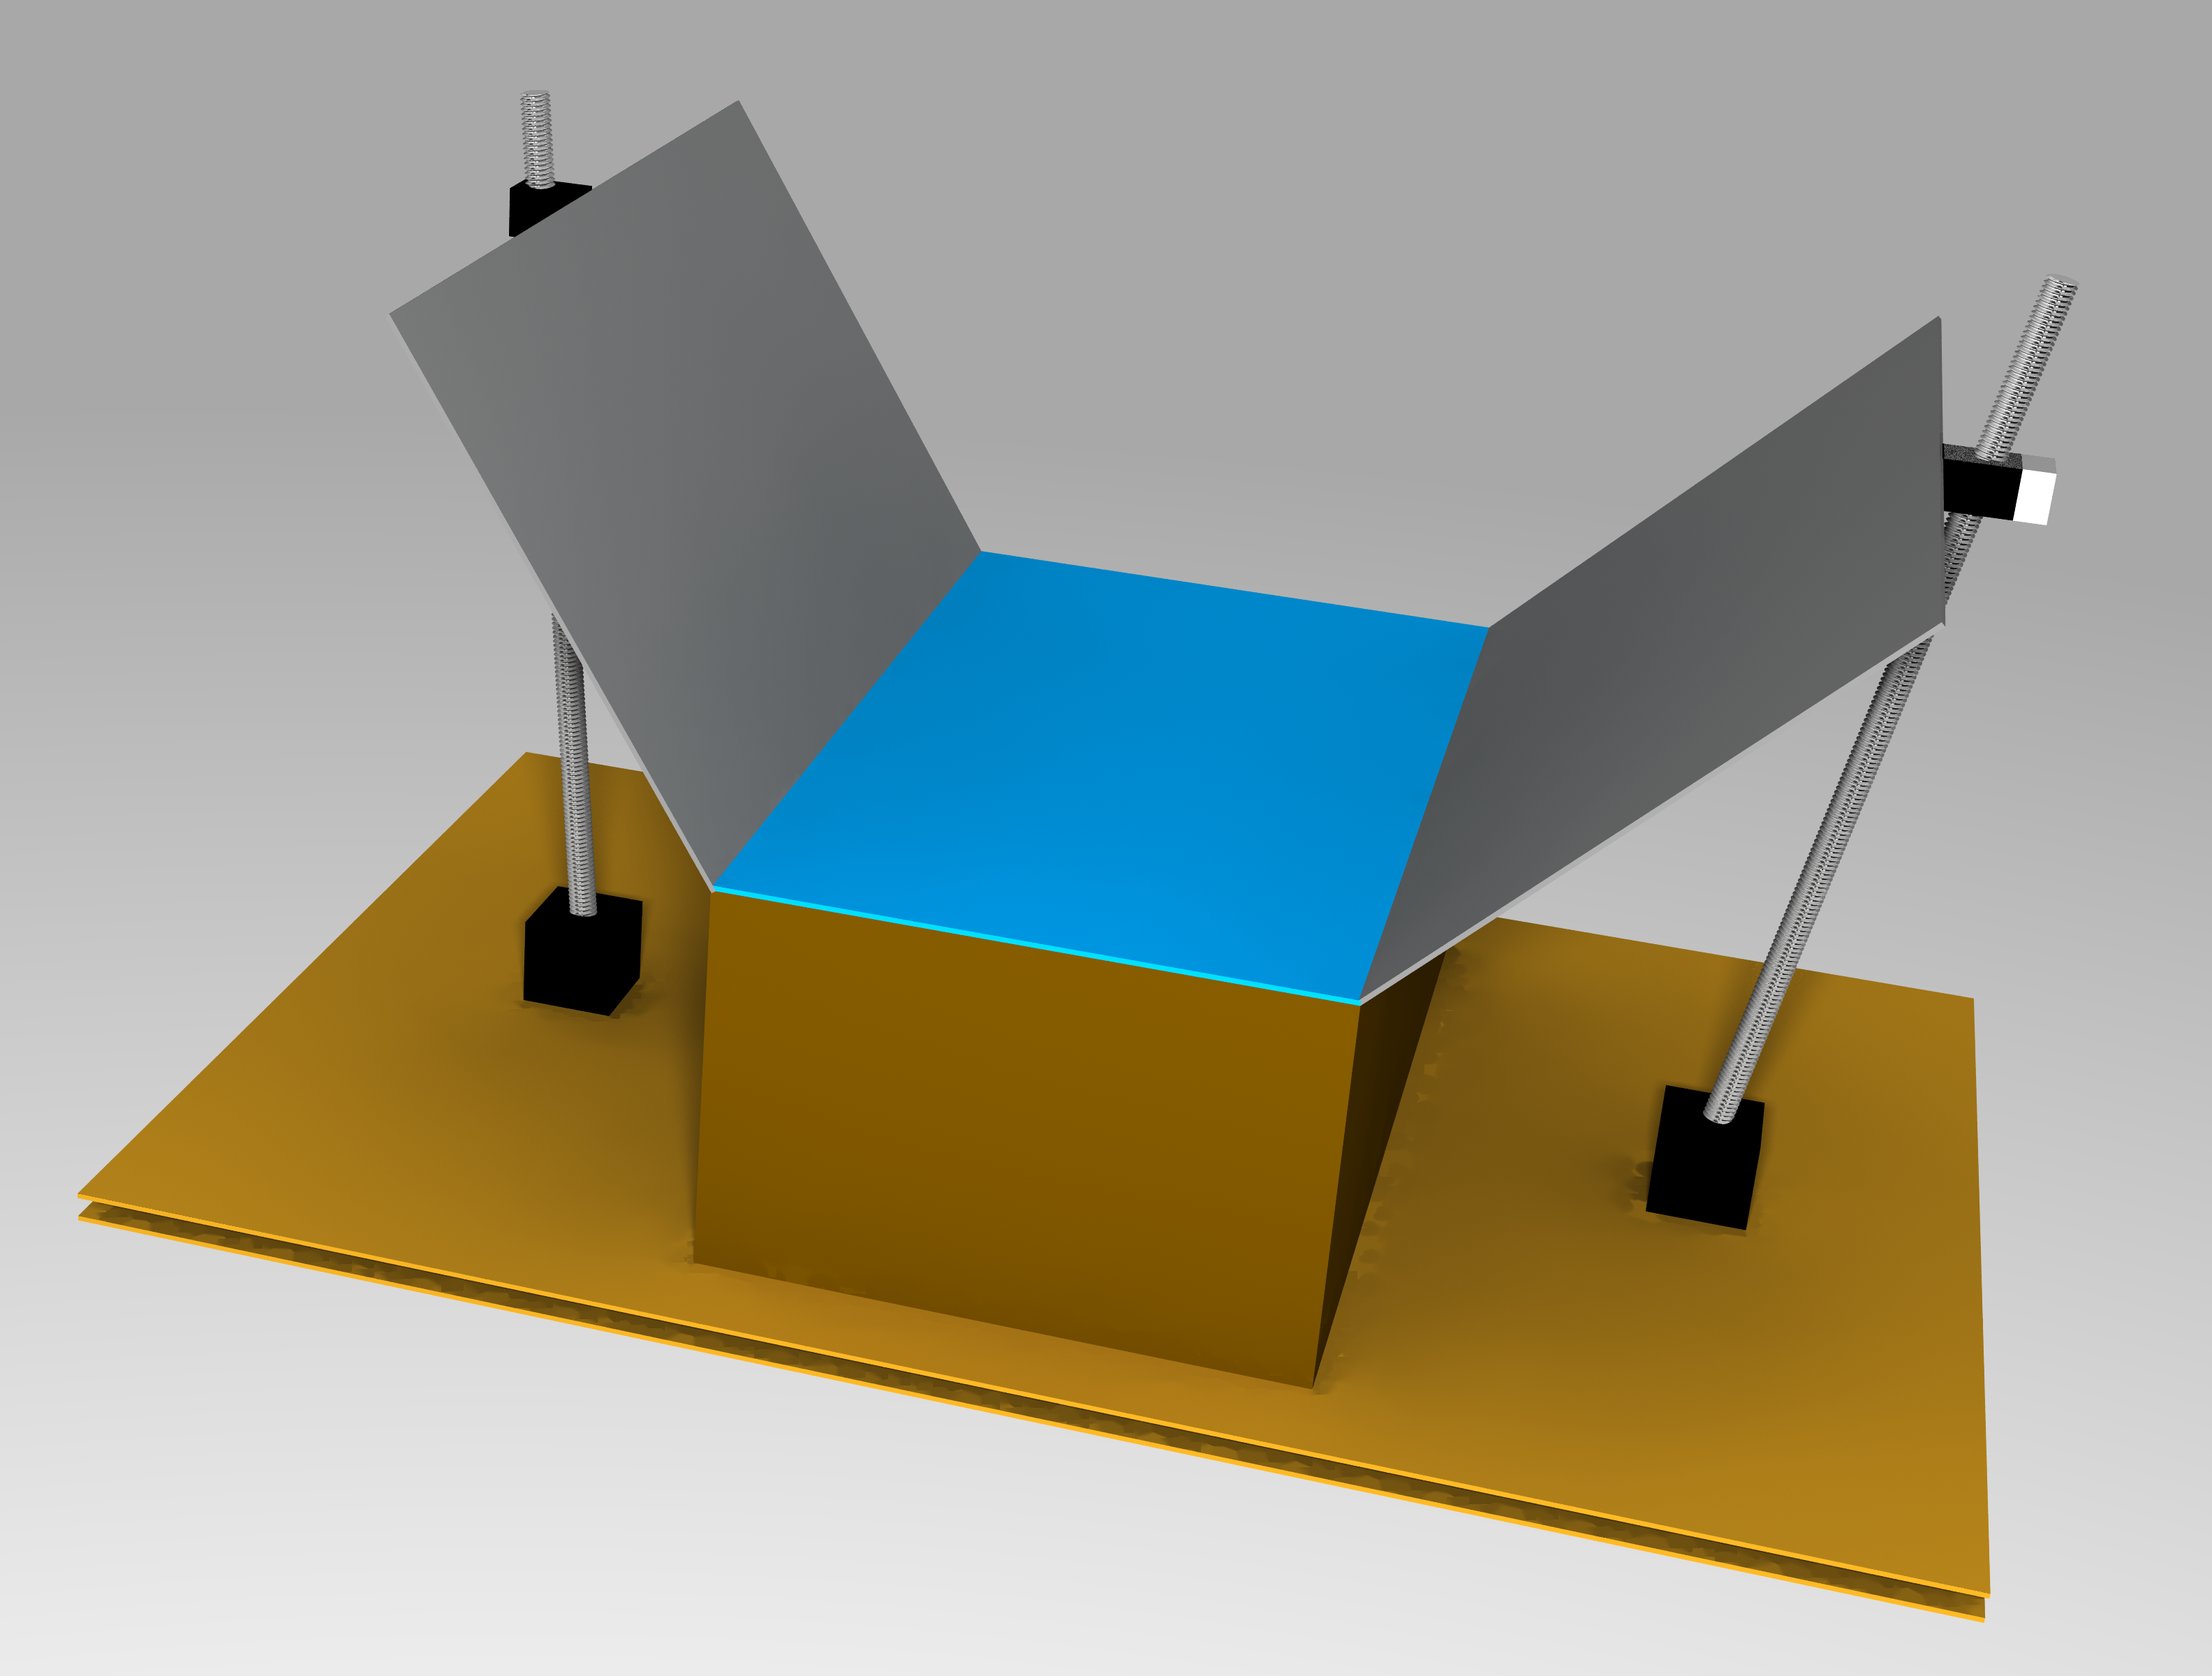
\includegraphics[width=380pt]{Draws/3D_render_cut.png}
        \caption{Modello generico struttura di base}
    \end{figure}
    
\section{Schema a blocchi}


\noindent
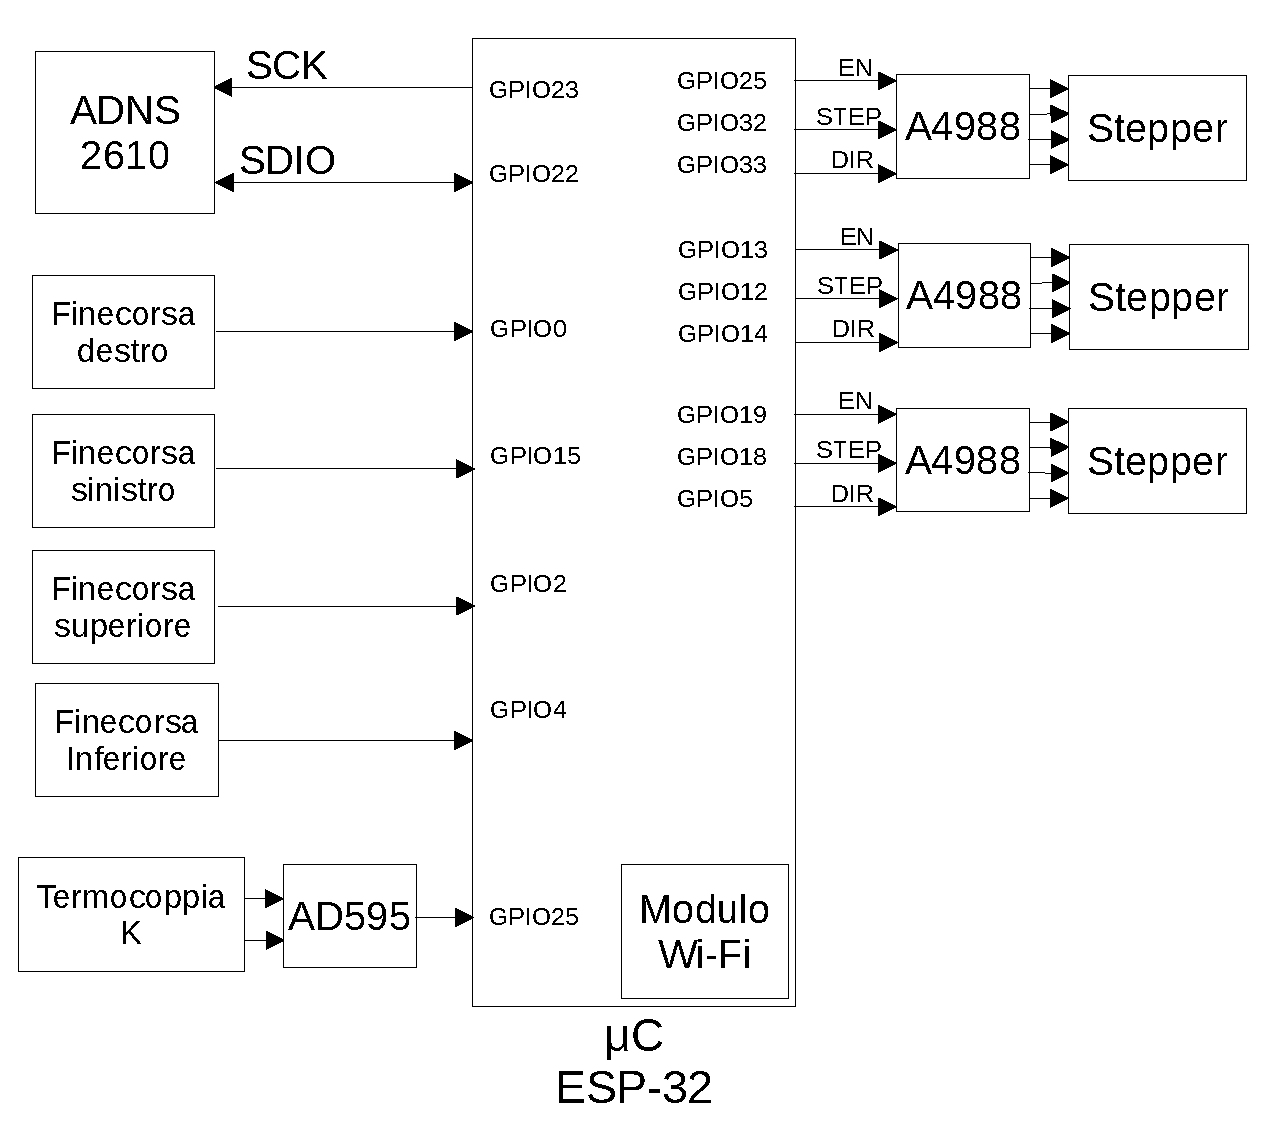
\includegraphics[
    page=1,
    width=\textwidth,
    height=\textheight,
    keepaspectratio
]{Draws/Block_diagram.pdf}

\noindent
Si assumono i finecorsa collegati in pulldown e con uscita allo stato alto quando premuti.\\

\vspace{0.3cm}
\noindent
I pin indicati a destra nel diagramma (GPIO25, GPIO32, GPIO33, GPIO13, GPIO12, GPIO14, GPIO19, GPIO18 e GPIO5) sono uscite, mentre i pin indicati a sinistra (GPIO23, GPIO0, GPIO15, GPIO2, GPIO4, GPIO25) sono input, unica eccezione il GPIO 22, che, come trattato in seguito nella sezione \ref{adns2610_protocol}, per la natura del protocollo seriale implementato dal sensore ADNS2610 richiede la possibilità di scambiare dati in modo bidirezionale.\\

\vspace{0.3cm}
\noindent
Il modulo Wi-Fi è interno al chip dell'ESP-32 e dunque non richiede collegamenti con i pin esterni.

\noindent


%Text below%\footnotemark[1]

\vfill



\section{Descrizione componenti}
    \subsection{Microcontrollore}
    Per la realizzazione di questo sistema di controllo è stato scelto di utilizzare un ESP-32, un microcontrollore a 32 bit con ingressi e uscite compatibili con la logica TTL.\\
    Questo microcontrollore (come il suo predecessore ESP8266) è spesso impiegato in applicazioni IoT, anche in ambito professionale, per la connessione wifi (e bluetooth per quanto riguarda l'ESP-32) integrata in un unico chip a basso costo, permettendo ai diversi dispositivi di comunicare tra loro.\\
    Per semplicità costruttiva di seguito ci si riferirà alla specifica implementazione me\-dian\-te la scheda di prototipazione rapida NodeMCU.
    
    \subsection{Motori}
    Dovendo regolare con accuratezza la rotazione dei motori, per il controllo di azimuth e inclinazione, si è deciso di impiegare dei motori passo-passo, o stepper, in particolare il modello NEMA-17.\\
    Questi attuatori sono motori ad impulsi, in quanto composti da bobine disposte in modo tale che, se eccitate in ordine opportuno, permettono di produrre una rotazione dell'asse inferiore a 1.8° per ogni step.\\
    Il principio di funzionamento è schematizzato nell'immmagine seguente.\\
    
    
    
    \begin{figure}[h]
    \centering
        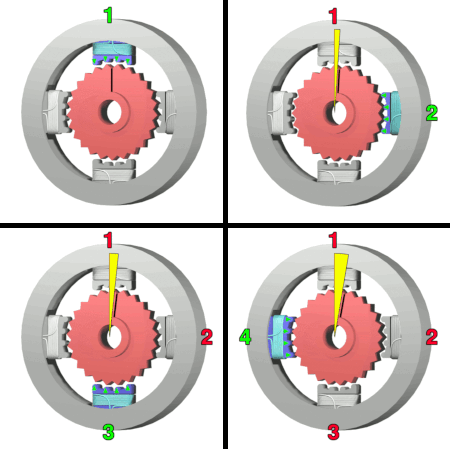
\includegraphics[width=300pt]{Draws/Animations/StepperMotor.png}
        \caption{Fasi motore passo-passo, Wikimedia Commons \protect\footnotemark}
    \end{figure}
    
    \vfill
    \footnotetext{Questa immagine è tratta e modificata da Wikimedia Commons, informazioni riguardo l'autore originale, modifiche successive e licenza GNU Free Documentation License possono essere reperite al seguente link: commons.wikimedia.org/wiki/File:StepperMotor.gif}
    
    
        \subsubsection{Controllo di potenza}
        Per il controllo dell'attivazione delle bobine si è scelto di utilizzare il modulo A4988 (molto diffuso nelle macchine a controllo numerico hobbistiche), che permette il controllo della rotazione del motore mediante un segnale di direzione (orario/antiorario) e un segnale di step.\\
        La logica di attivazione degli avvolgimenti del motore è gestita dell'integrato mediante due ponti H a fet, uno per bobina, che permettono la regolazione della potenza ad ogni avvolgimento.\\
        Il funzionamento interno, come mostrato dal costruttore nel datasheet, può essere schematizzato con il seguente diagramma a blocchi.\\
        \begin{figure}[h]
        \centering
            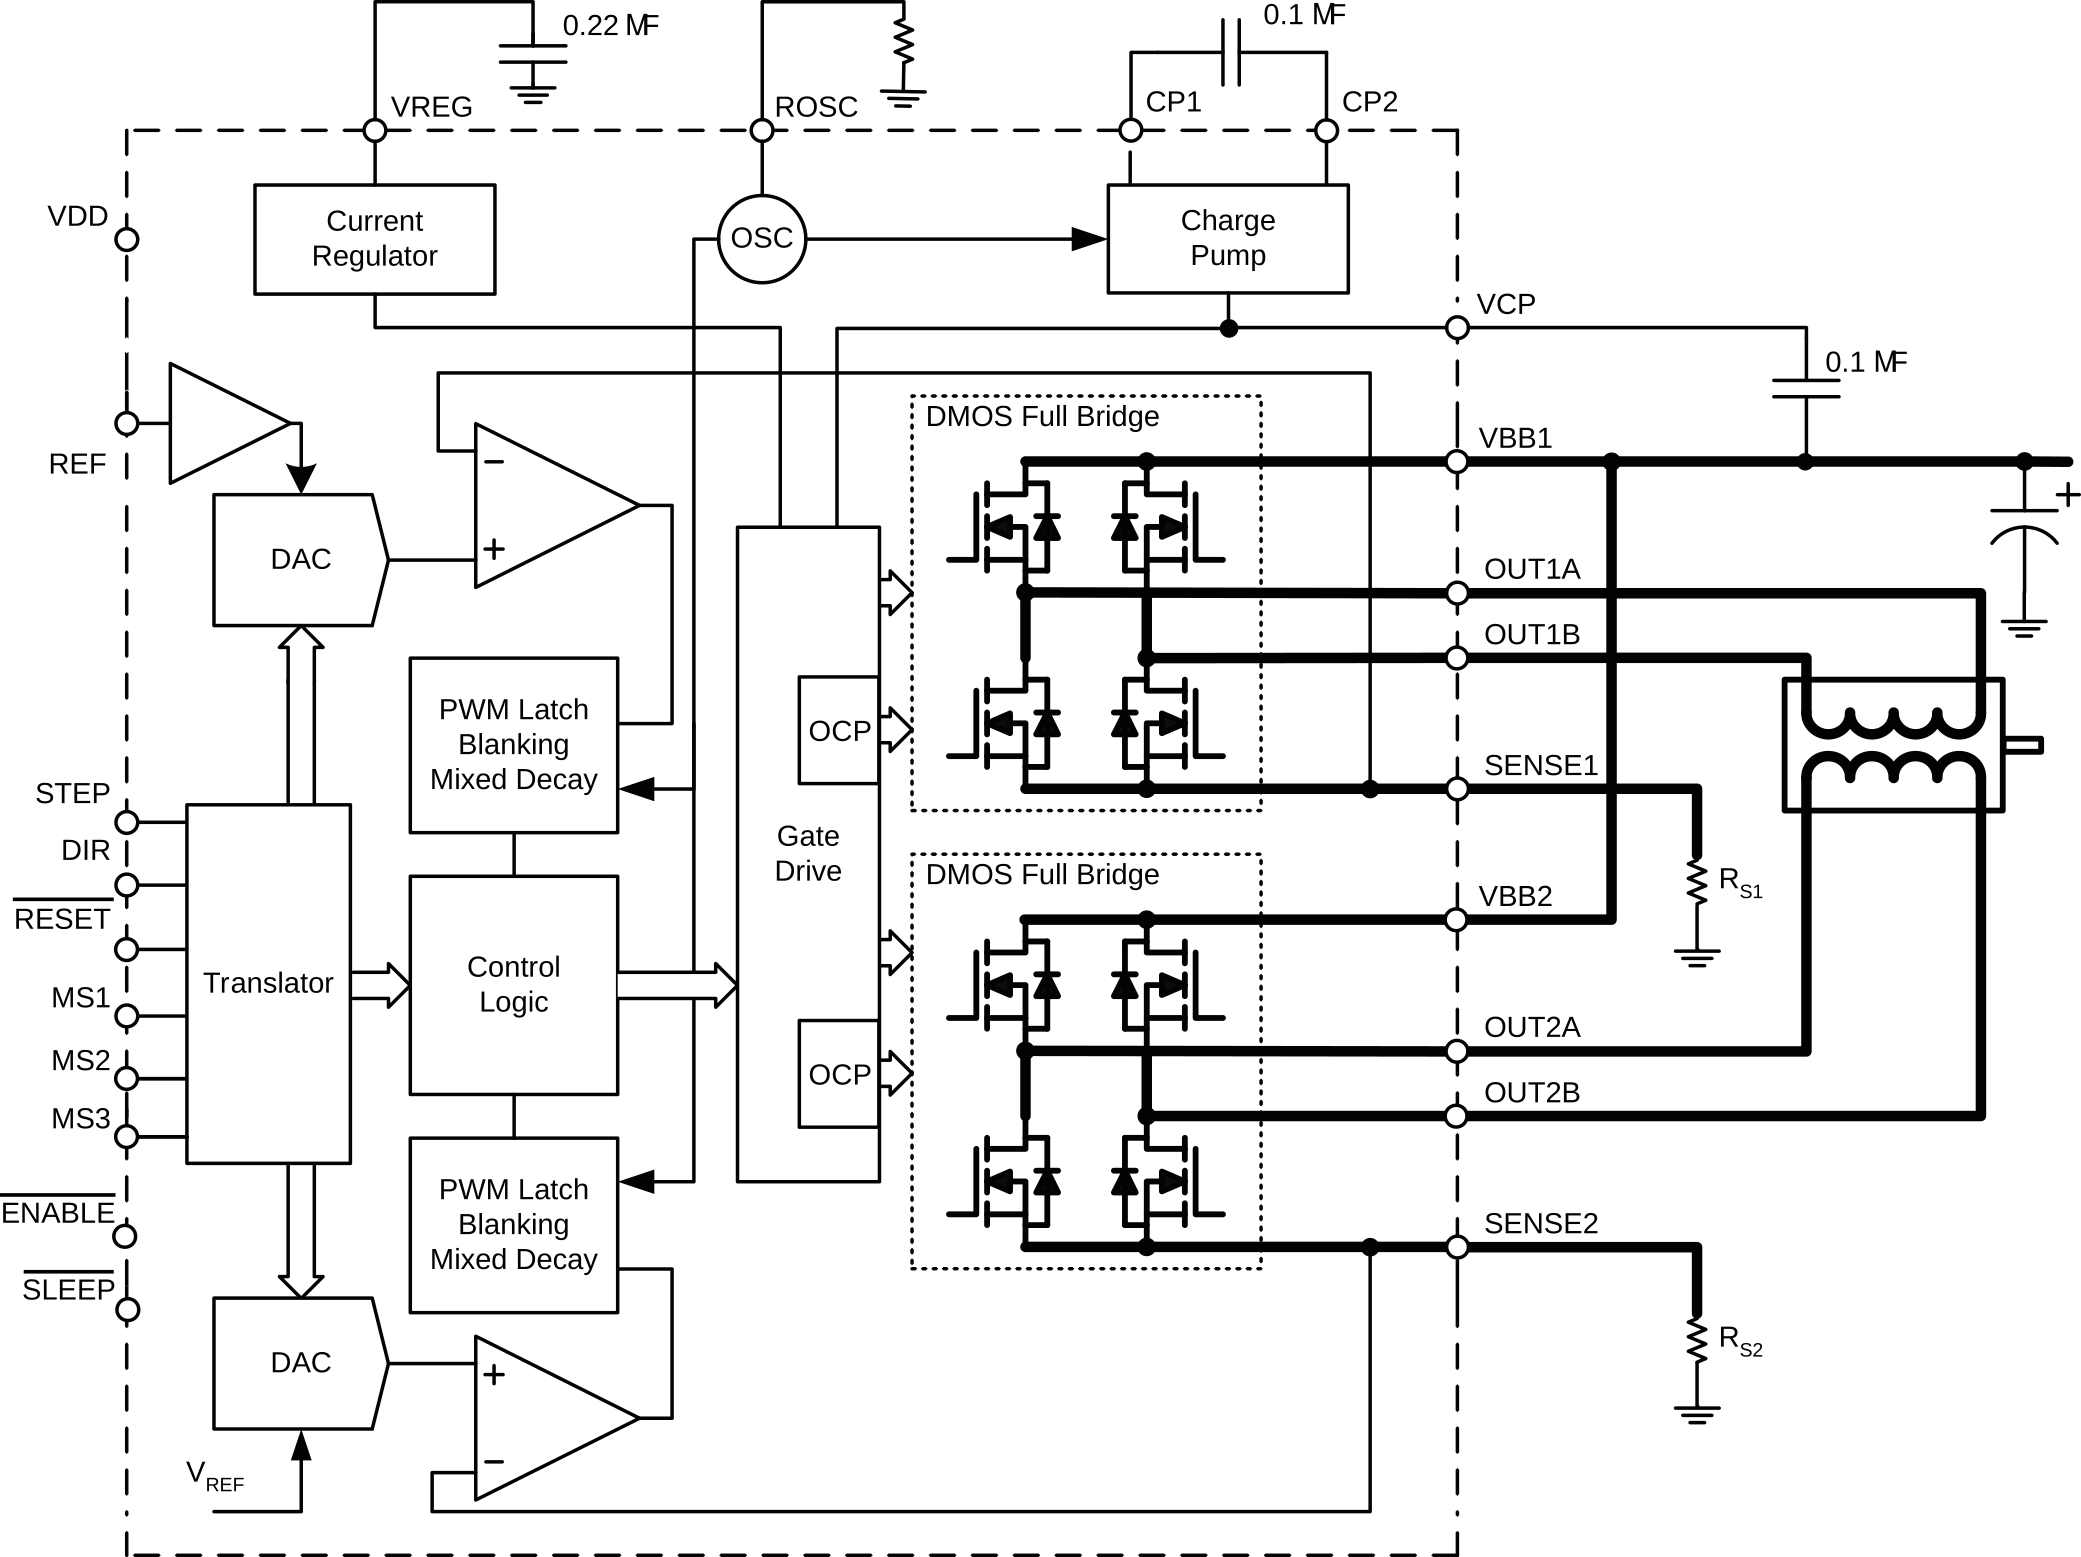
\includegraphics[width=370pt]{Draws/A4988_functional_diagram.png}
            \caption{Diagramma funzionamento interno A4988, datasheet}
            \label{fig:A4988_diagram}
        \end{figure}
        
        \noindent
        Gli ingressi $MS_1$, $MS_2$ e $MS_3$ permettono la selezione del rapporto di microstepping, infatti oltre alla modalità full-step, in cui le singole bobine vengono eccitate con controllo ON-OFF in successione, è possibile realizzare un controllo micro-stepping con l'attivazione progressiva delle bobine consecutive, permettendo di mantenere il rotore tra due stati successivi, garantendo una maggiore fluidità di movimento, riducendo oscillazioni, vibrazioni e dunque sollecitazioni meccaniche della struttura fisica.\\
        Con riferimento all'immagine di Fig. \ref{fig:A4988_diagram} si può osservare che il dispositivo permette di regolare la coppia massima del motore mediante la regolazione di una tensione di riferimento che agisce sulla corrente massima che viene fornita alle bobine (misurata dalle resistenze di shunt $R_{s1}$ e $R_{s2}$ che forniscono un feedback al sistema di controllo).

        \vspace{0.1cm}


    \subsection{Termocoppia}\label{thermocouple}
    Per la rilevazione della temperatura si è scelto di utilizzare una termocoppia di tipo K a giunzione Chromel-Alumel (leghe metalliche a base di nichel), sensore molto diffuso che premette di misurare temperature nel range da circa -200 °C a oltre 1300 °C, con una sensibilità di $41 \frac{\mu V}{\degree C}$.\\
    Le termocoppie sfruttano l'effetto Seebeck, un effetto termoelettrico che produce una differenza di potenziale tra due punti di un materiale conduttore proporzionale alla differenza di temperatura tra i due punti (detti guinzione calda e giunzione fredda); l'intensità di questo effetto varia a seconda del materiale in considerazione e quindi, utilizzando due maetalli differenti, è possibile calcolare la temperatura del giunto caldo nota la differenza di potenziale e la temperatura del giunto freddo.\\
    Per rendere apprezzabili tali variazioni di tensione è necessario impiegare un amplificatore da strumentazione, in particolare si è scelto l'AD595, che garantisce la compensazione interna della temperatura della giunzione fredda e fornisce in uscita una tensione proporzionale alla tempreatura secondo la relazione:
    \begin{equation}\label{thermocouple_relation_AD595}
        V_{out} = T \cdot 10 \frac{mV}{\degree C}
    \end{equation}
    Nella sezione \ref{conditioning} si tratterà più approfonditamente il condizionamento di questo segnale per sfruttare l'intero range dell'ADC del microcontrollore.
    
    
    \subsection{Sensore ottico}\label{optical_sensor}
    Il sensore principale di questo sistema di controllo è l'ADNS-2610, che viene utilizzato dal microcontrollore per calcolare l'azimuth e l'elevazione relativi del sole.\\
    
    \begin{figure}[h]
        \centering
        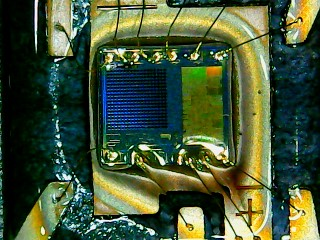
\includegraphics[width=250pt]{Draws/ADNS-2610_die/WIN_20210501_17_42_53_Pro.jpg}
        \caption{Sensore ADNS-2610}
        \label{fig:ADNS2610_die}
    \end{figure}
   
    \noindent
    Questo integrato nasce come sensore per mouse ottici, che dispongono di una fotocamera a bassa risoluzione e confrontano le immagini di due frame successivi per individuare lo spostamento relativo alla superficie sottostante, nella porzione di sinistra della figura \ref{fig:ADNS2610_die} si osserva la matrice 18x18 degli elementi fotosensibili (l'immagine è stata realizzata con un ingrandimento e l'area effettiva coperta dalla griglia è di circa 2 $mm^2$).\\
    Il principio di funzionamento è identico ad una camera a foro di spillo, in cui l'immgine viene proiettata sullo schermo fotosensibile attraverso un foro circolare di piccole dimensioni.
    
    \begin{figure}[h]
        \centering
        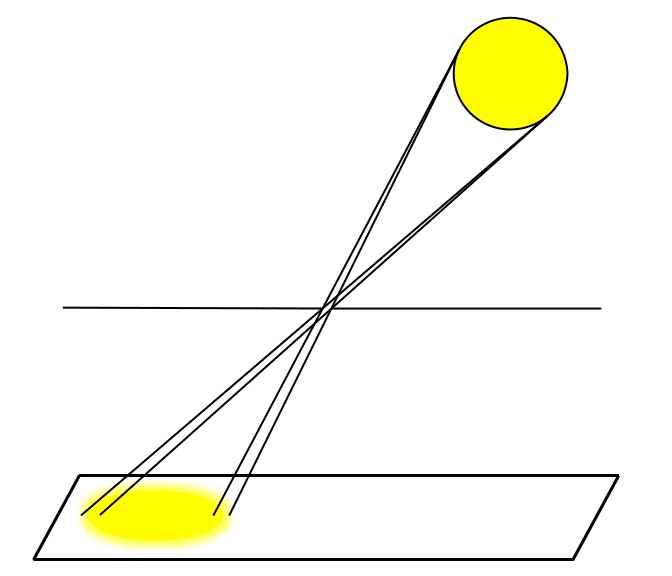
\includegraphics[width=150pt]{Draws/Pinhole_sun}
        \caption{Schema immagine stenoscopica}
        \label{fig:pinhole_sun}
    \end{figure}
    
    \noindent
    La posizione dell'immagine sullo schermo, a parità delle altre condizioni, varia al variare della distanza tra il foro e il sensore stesso, in particolare, aumentando tale distanza il dispositivo avrà un angolo di campo minore, viceversa, diminuendo la distanza foro-rivelatore, si otterrà un angolo di campo maggiore.
    
    \begin{figure}[h]
        \centering
        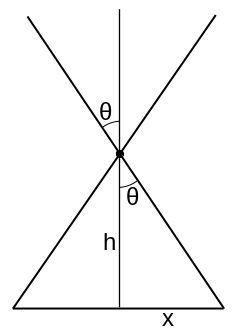
\includegraphics[width=110pt]{Draws/Pinhole_diagram}
        \caption{Diagramma camera a foro di spillo}
        \label{fig:pinhole_diagram}
    \end{figure}
    
    \noindent
    In cui la relazione tra $x$ e l'angolo $\theta$ del raggio rispetto allo zenit è:
    \begin{equation}\label{pinhole_angle_relation}
        x = h \cdot tan(\theta)
    \end{equation}
    
    \noindent
    Maggiori dettagli riguardo l'interfacciamento in protocollo con il microcontrollore sono forniti nella sezione \ref{adns2610_protocol}.
    
    %\subsection{Interfaccia web}
    
 
\section{Condizionamento segnale sensore temperatura}\label{conditioning}
    Considerata l'uscita del AD595 descritta dall'equazione (\ref{thermocouple_relation_AD595}) nella sezione \ref{thermocouple} e considerata la risoluzione di 12 bit degli ADC del microcontrollore, si ottiene una minima variazione apprezzabile (idealmente) inferiore a 0.12 °C. Per questo motivo non è necessario realizzare un secondo condizionamento del segnale, in quanto tale valore di incertezza è trascurabile rispetto alle temperature da misurare e alle altre fonti di errore presenti; per maggiore completezza si riporta comunque un possibile condizionamento di tale segnale. \\
    
    \vspace{0.2cm}
    
    \noindent
    Si limiti il range di interesse da 15°C a 300°C in cui rientra la regolare temperatura di un forno solare.\\
    Secondo la relazione (\ref{thermocouple_relation_AD595}) l'uscita in tensione del sensore varierà all'interno dell'intervallo [150mV; 3.0V], mentre l'ADC integrato nel microcontrollore, con $V_{ref}$ standard, ammette ingressi nel range [0V; 3.3V]; di seguito si suppongono tutti i dispositivi impiegati come ideali.\\
        È possibile applicare un offset di 
        \begin{equation}\label{offset}
            {V_{offset}} = V_{Smin} - V_{ADCmin} = 150 mV
        \end{equation}
        e successivamente un'amplificazione di
        \begin{equation}\label{amplification}
            A = \frac{V_{ADCmax}-V_{ADCmin}}{V_{Smax} - V_{Smin}} \simeq 1.16
        \end{equation}
        utilizzando un amplificatore operazionale in configurazione differenziale come segue.

        \noindent
        \begin{center}
            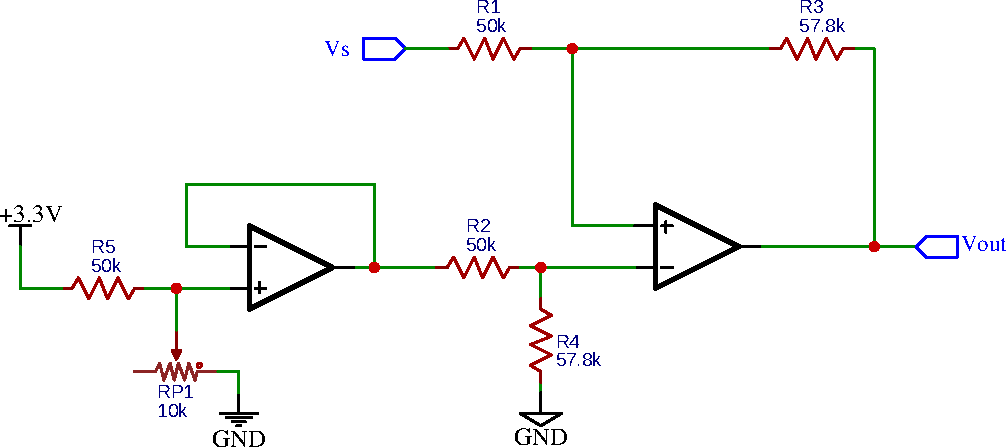
\includegraphics[
                page=1,
                width=\textwidth-120pt,
                keepaspectratio
            ]{Draws/Schematic_Elaborato_2021-05-15_differential.pdf}
        \end{center}
                
        \noindent
        In cui il potenziometro (o trimmer) $RP_1$ deve essere opportunamente regolato in fase di calibrazione per ottenere l'offset corretto.\\
        Essendo $R_1=R_2$ e $R_3=R_4$ l'amplificazione risulta $A = \frac{R_3}{R_1} \simeq 1.16$, stesso valore ottenuto sostituendo i rispettivi valori numerici nell'equazione (\ref{amplification}). Riguardo alle due resistenze da $57.8 k\Omega$, tale può essere ottenuto dalla serie di una resistenza da $56 k\Omega$ e da $1.8 k\Omega$, entrambi valori appartenenti alla serie E12.\\
        Combinando le equazioni (\ref{thermocouple_relation_AD595}), (\ref{offset}) e (\ref{amplification}), la funzione di trasferimento dell'amplificatore differenziale e considerata la conversione dell'ADC a 12 bit dell'ESP-32 (valore da 0 a 4095), si ottiene:
        \begin{equation}
            Val_{ADC} = \left( T \cdot 10 \left[ \frac{mV}{\degree C} \right] - 150 [mV] \right) \cdot \frac{57.8}{50} \cdot \frac{4095}{3.3[V]} \simeq \left( \frac{T}{1 [\degree C]} - 15 \right) \cdot  14.345
        \end{equation}
        
        \noindent
        chiaramente approssimato all'intero, da cui si ricava
        
        \begin{equation}
            T = \left( \frac{Val_{ADC}}{14.345} + 15 \right) [\degree C]
        \end{equation}
    
        \noindent
        L'aggiunta di questo condizionamento richiede inoltre ulteriori componenti per la generazione dell'alimentazione duale per l'operazionale, quindi, in aggiunta a quanto già discusso all'inizio di questa sezione, non è stato ritenuto necessario impiegare condizionamenti successivi all'integrato AD595.
\vspace{1cm}

\section{Cenni matematici}
    \subsection{Sistema coordinate cartesiane - polari}
    Si ricorda che è possibile definire in modo univoco un punto A sul piano cartesiano mediante le sue coordinate $(x_A, y_A)$. Lo stesso punto A può anche essere descritto univocamente dalla distanza $r$ dal centro e dall'angolo $\alpha$ che esso forma con il centro e il semiasse positivo delle ascisse.
    
    \begin{figure}[h]
    \centering
        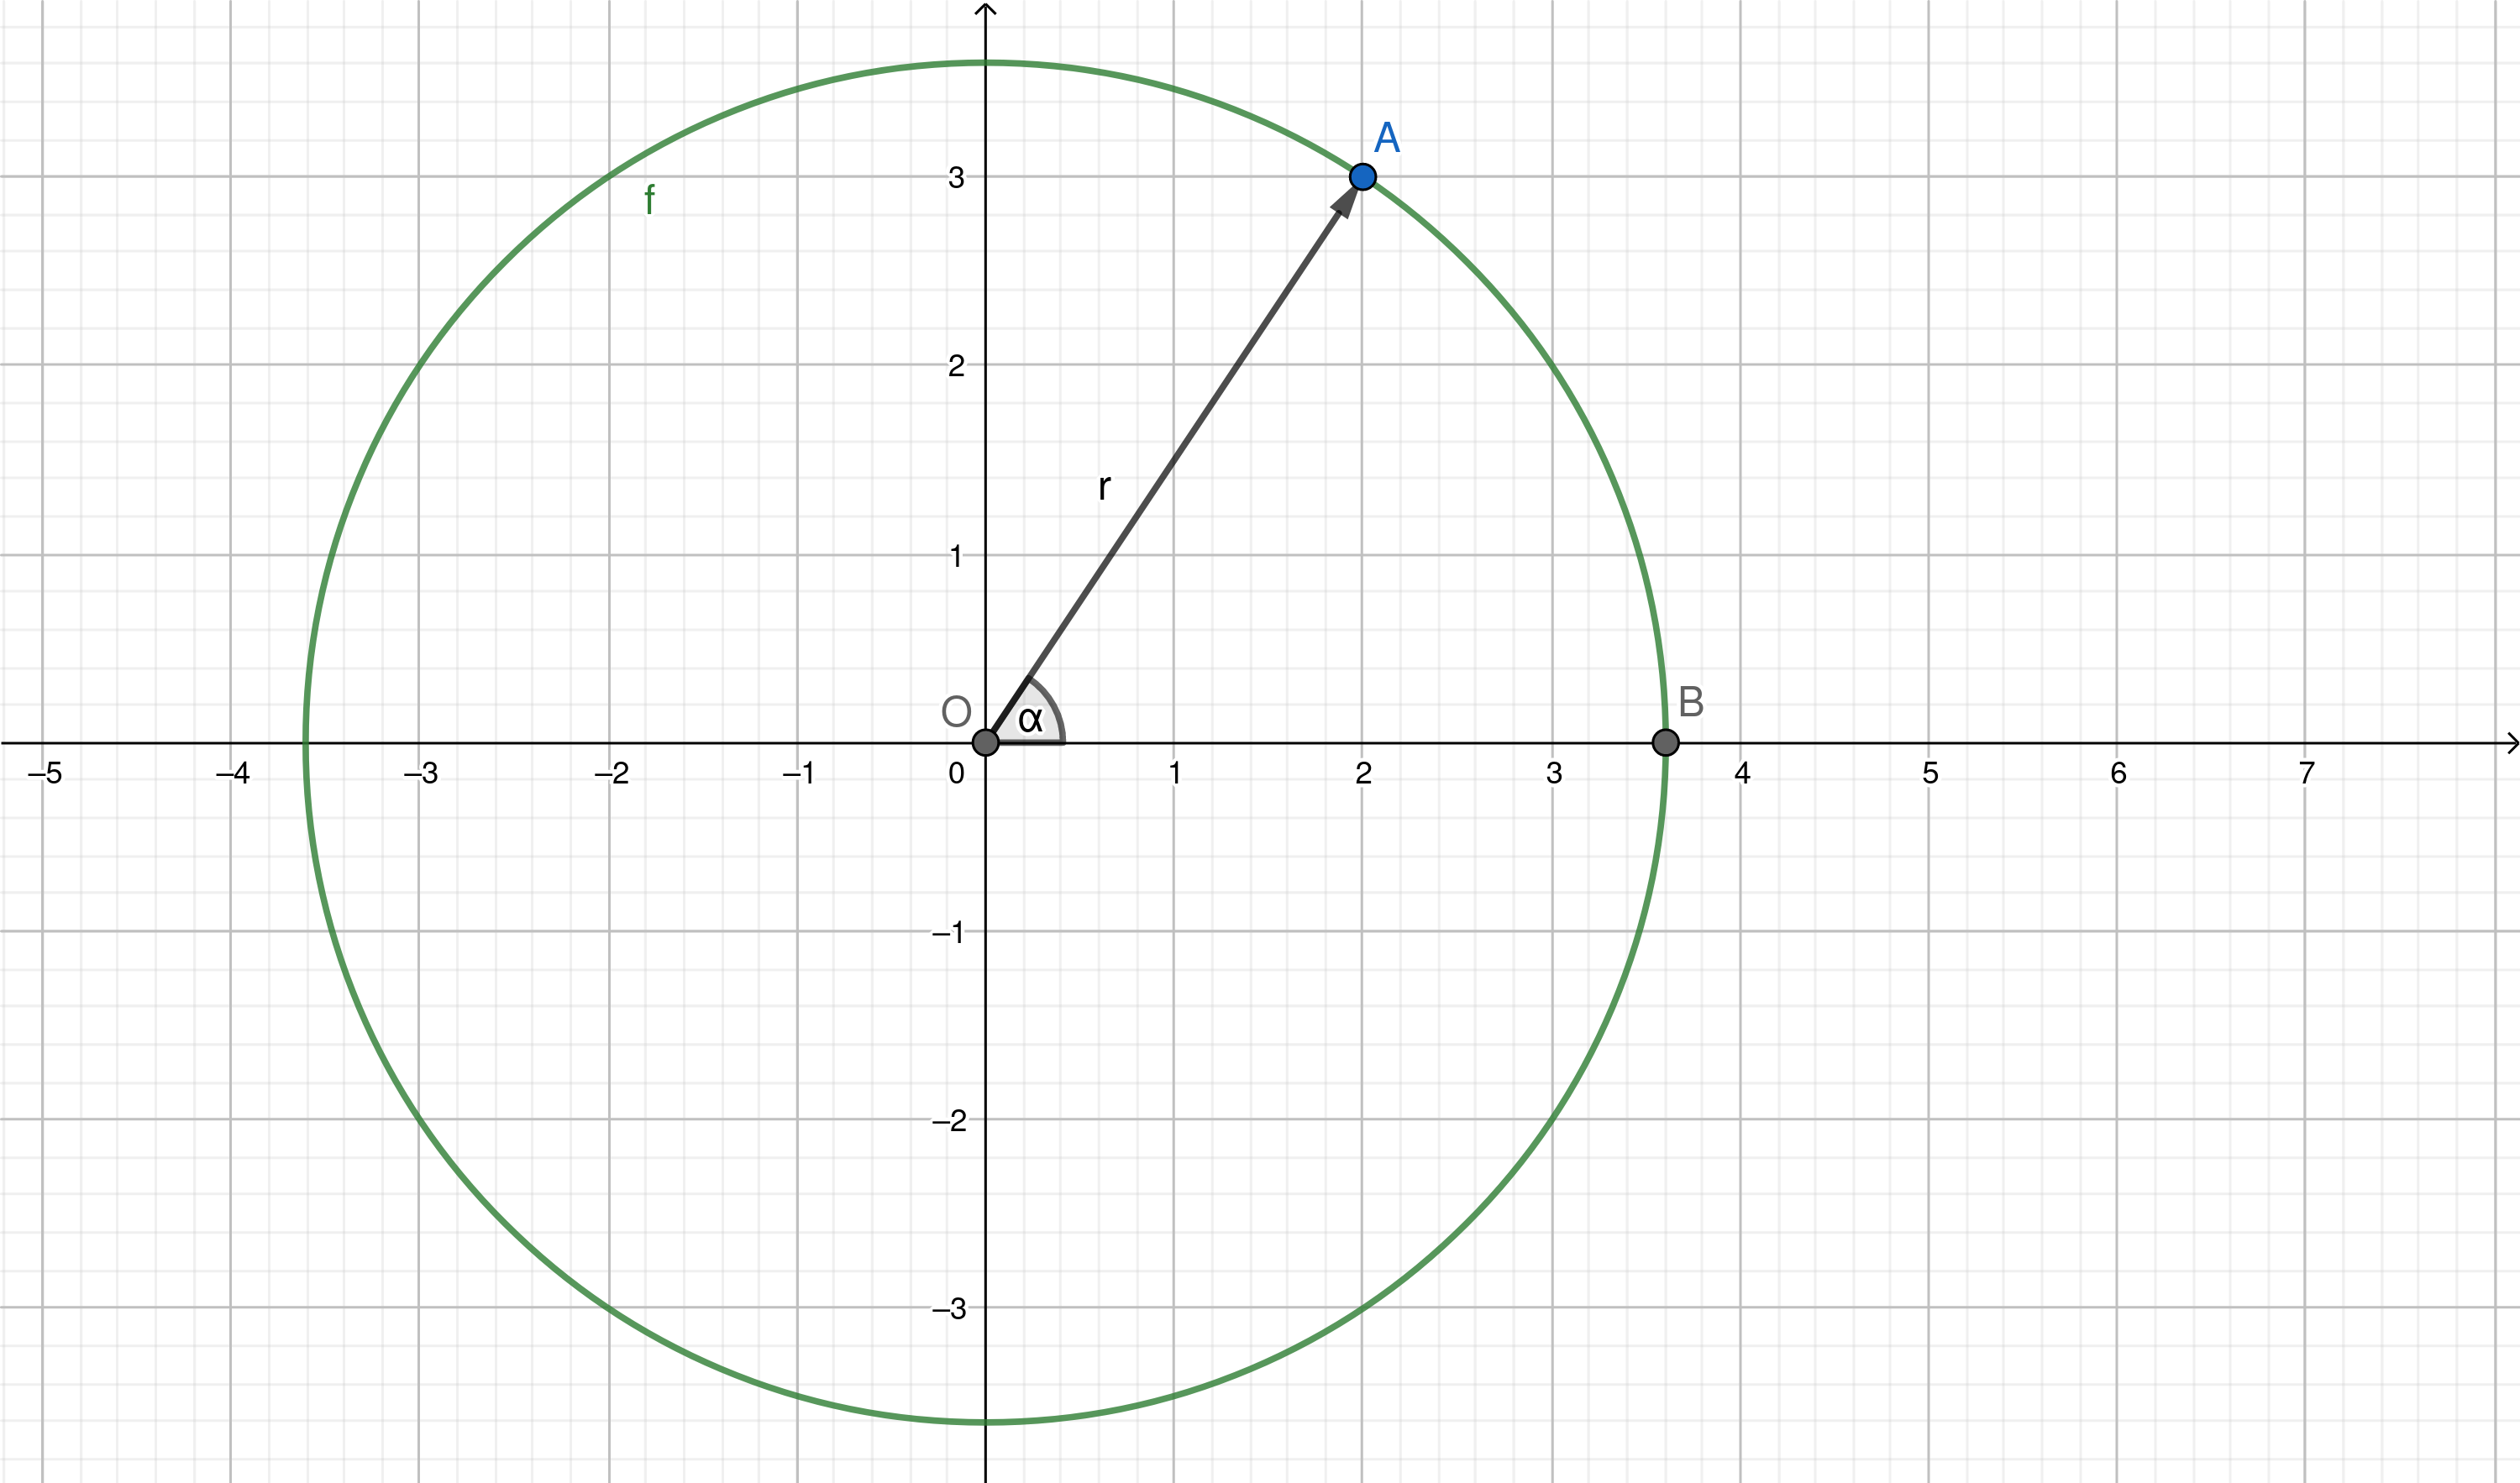
\includegraphics[width=300pt]{Draws/geogebra-export_polar_circle.png}
        \caption{Rappresentazione coordinate polari su piano cartesiano, geogebra}
    \end{figure}
    
    \noindent
    È possibile ottenere la rapprentazione cartesiana dalle coordinate polari secondo le relazioni:
    
    \begin{equation}
        \begin{split}
        x_A = r \cdot \cos\alpha \\
        y_A = r \cdot  \sin\alpha
        \end{split}
    \end{equation}
    
    \noindent
    Viceversa:
    
    \begin{equation}
        \begin{split}
        r = \sqrt{x_A^2 + y_A^2} \\
        \alpha = atan \left(\frac{y_A}{x_A} \right)
        \end{split}
    \end{equation}
    
    \noindent
    In particolare, una volta determinata la posizione del centro del sole nell'immagine acquisita, ed espresso tale punto in coordinate polari $(r, \alpha)$, $r$ è direttamente legato all'elevazione effettiva del sole secondo la relazione (\ref{})
    
    
    \subsection{Relazioni trigonometriche}

\section{Algoritmo}
    \subsection{Diagramma di flusso generale}

    \subsection{Analisi funzioni principali}
        \subsubsection{Controllo accelerazione motori}
        \subsubsection{Protocollo sensore ottico}\label{adns2610_protocol}
        \subsubsection{Calcolo gradiente}
        
        
        \subsubsection{Discesa del gradiente}
        Per ottenere il centro dell'immagine del sole, che approssimiamo ad un cerchio, è sufficiente trovare la circonferenza che meglio approssima il contorno esterno del cerchio, definito dai punti con maggiore modulo del gradiente, ovvero in cui si ha una differenza netta tra pixels successivi. \\
        A tal fine si deve minimizzare la distanza geometrica tra la circonferenza e i punti con magiore modulo del gradiente; tale distanza è schematizzata nella seguente figura con il tratto $ e $.
        
        \begin{center}
        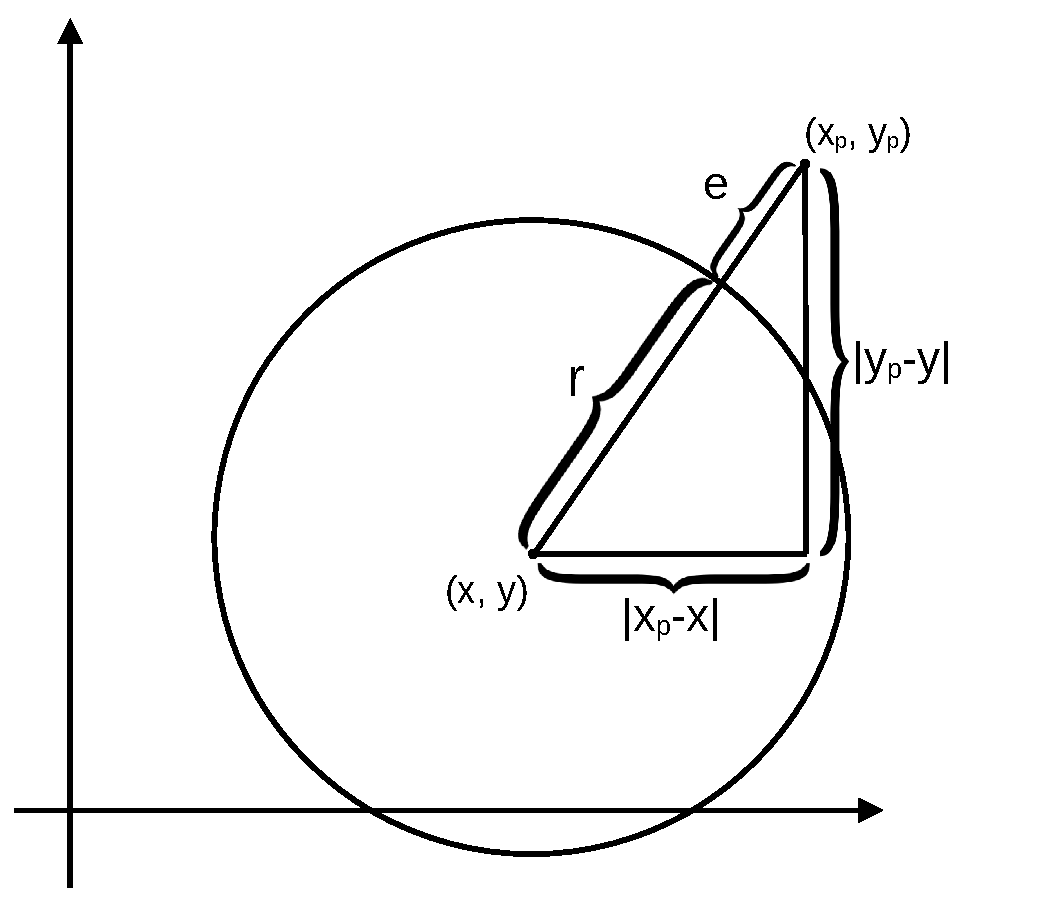
\includegraphics[
            page=1,
            width=220pt,
            height=\textheight,
            keepaspectratio
        ]{Draws/Discesa_del_gradiente_cerchio-punto.pdf}
        \end{center}
        
        \noindent
        Applicando il teorema di pitagora, per differenza, si ottiene che la distanza $ e $ è definita in funzione delle coordinate del centro e del punto in questione, secondo la relazione
        \begin{equation}
             e = \left| \sqrt{(x_p-x)^2 + (y_p-y)^2} -r \right|
        \end{equation}
        
        \noindent
        Possiamo quindi definire la seguente funzione
        \begin{equation}
            f(x, y, r) = \sum_{y_p = 0}^{15} \sum_{x_p = 0}^{15} \left[ g(x_p, y_p) \cdot \left| \sqrt{(x_p-x)^2 + (y_p-y)^2} -r \right| \right] 
        \end{equation}
        
        \noindent
        in cui la funzione $ g(x_p, y_p) $ rappresenta il modulo del gradiente dell'immagine del punto $ (x_p, y_p) $, ed è quindi un coefficiente reale. Tale sommatoria risulta quindi una somma ponderata delle distanze tra la circonferenza in considerazione e tutti i punti della matrice discussa alla sezione precedente. Il modulo del gradiente sarà maggiore per i punti sul contorno dell'immagine del sole, che quindi avranno un peso maggiore rispetto agli altri punti.\\
        Calcoliamo quindi le derivate parziali di $ f(x, y, r) $ rispetto alle tre variabili
        
        \begin {equation}
            \frac{\partial f}{\partial x} = \sum_{y_p = 0}^{15} \sum_{x_p = 0}^{15} \left[ g(x_p, y_p) \cdot sgn \left( \sqrt{(x_p-x)^2 + (y_p-y)^2} - r \right) \cdot \frac{x - x_p}{\sqrt{(x_p - x)^2 + (y_p - y)^2}} \right] 
        \end {equation}
        \begin {equation}
            \frac{\partial f}{\partial y} = \sum_{y_p = 0}^{15} \sum_{x_p = 0}^{15} \left[ g(x_p, y_p) \cdot sgn \left( \sqrt{(x_p-x)^2 + (y_p-y)^2} - r \right) \cdot \frac{y - y_p}{\sqrt{(x_p - x)^2 + (y_p - y)^2}} \right] 
        \end {equation}
        \begin {equation}
            \frac{\partial f}{\partial r} = \sum_{y_p = 0}^{15} \sum_{x_p = 0}^{15} \left[ - g(x_p, y_p) \cdot sgn \left( \sqrt{(x_p-x)^2 + (y_p-y)^2} - r \right) \right] 
        \end {equation}
        
        \noindent
        con $ sgn(x)$ definita a tratti nel dominio $(- \infty ; 0) \cup (0; +\infty) $ :
        
        \begin {equation}
            sgn(x) = 
                \begin{cases}
                  -1 & \text{se x < 0} \\
                  1 & \text{se x > 0}
                \end{cases}
        \end {equation}
        

\/*
    \begin{changemargin}{-1cm}{-1cm}

    \lstinputlisting{Sketch_simulazione_elaborato_serra/Sketch_simulazione_elaborato_serra.ino}
    \end{changemargin}
*/    
  
   
    \vfill
    \let\thefootnote\relax\footnotetext{
        \begin{center}
            Documento realizzato in \LaTeX.
        \end{center}
    }
\end{document}

